\chapter{Model Training}
\label{chap:tuning}

In this chapter, we describe the process of developing
the statistical post-editing models. We take a closer look at the task of model
selection and parameter tuning, the feature selection methods we have experimented
with and several methods of evaluation used during the tuning.
We only present experiment results for the separate statistical models,
evaluation of the whole MLFix system is presented in the next chapter.

In this chapter, we cover the following two classification tasks: the identification
of incorrect instances (words from the MT output with incorrect surface form),
addressed as \pojem{error detection} for short,
and the prediction of the new morphological categories for the incorrect instances,
referred to as \pojem{morphological prediction}.

Our development process can be separated into three stages: in the first stage, we
have focused on basic comparison of different ML methods and choice of the most
suitable candidate for each task.
In the second stage we have tried to further increase the performance of the model
based on the chosen ML method by experimenting with various methods for feature selection
and in the third stage, for each dataset, we have searched for the best hyperparameters
of the both the selected ML method and the feature filtering method.

\section{Model Evaluation Methodology}

We have decided to do word-level evaluation during the model development. More precisely,
we have evaluated performance of models using the instances extracted by the
process we have described in the previous chapter.

For both error detection and morphological prediction task, we have defined
a baseline model for comparison. The baseline model basically represents a predictor which
does not detect any errors (all instances are marked as correct) or keeps the original
morphological categories for each instance.

Aside from a standard accuracy metric, we have also measured
precision and recall
of the models we trained to gain additional information about the model performance.
We use standard definition of precision~(\ref{eq:prec-mod}) and recall~(\ref{eq:rec-mod}) computed using the following equations:
\begin{equation} \label{eq:prec-mod}
precision = \frac{TP}{TP + FP}
\end{equation}
\begin{equation} \label{eq:rec-mod}
recall = \frac{TP}{TP + FN}
\end{equation}
However, we have slightly altered the definitions of \pojem{true positives} (TP),
\pojem{false positives} (FP) and \pojem{false negatives} (FN)
with regard to the baseline model.

%vary slightly with each classification task. We also use F-measure to compare combined results of these metrics.

For error detection, each instance that was assigned the same value as the \pojem{true prediction}
and a different value than the \pojem{baseline} is marked as TP. Eash instance
that was assigned a value different from both the \pojem{true prediction} and the \pojem{baseline}
is marked as FP and each instance with the \pojem{predicted value} equal to the \pojem{baseline}
but different from the \pojem{true prediction} is marked as FN.

For morphological prediction, we use the same definition of TP, however, the definitions
of FP and FN are altered in the following way (the \pojem{true prediction}
does not match the \pojem{predicted value}):
\begin{itemize}
\item if the \pojem{baseline} value matches the \pojem{predicted value}, an instance is marked as FN,
\item if the \pojem{baseline} value matches the \pojem{true prediction}, an instance is marked as FP,
\item if the \pojem{baseline} does not match either one, an instance is marked as \pojem{wrong positive} (WP).
\end{itemize}

The WP is a special case which reflects the situation where predictor tries to predict new value (different
from the original one) but fails and returns just another incorrect value.

We must also take into account
that the error detection classifier is a general model, which is not designed to distinguish
the types of morphological errors and the morphological predictor might be specialized only on a limited
set of the morphological categories. Therefore, sometimes we want the morphological predictor to just leave the \equo{incorrect}
instances unchanged because it is simply incapable of predicting new values of the incorrect categories.

In the end, we have found the basic accuracy metric to be more informative for evaluating the morphological predictor,
not only because in takes the WP instances into account but also due to the nature of our training data. We use only instances
that are marked as incorrect by our heuristic
which make precision/recall less relevant compared to accuracy.
On the other hand, if we decided to expand our training data
by \equo{correct} instances, these metrics would become more useful. 

\section{Automatic Error Detection}

%data rep - # of features
%cv method
%baseline

As we have already pointed out, 
the task of identifying morphologically incorrect words in the text is more difficult
than the task of assigning new morphological categories. It is not surprising
that we have faced several issues
during the development which we describe in more detail in the following sections.



\subsection{Unbalanced Data Problem}

In this task, we face the problem of binary classification, where we
assign the value 0 to instances that we consider correct (they are not going to change) and the value 1 to
instances that need to be corrected. The process of assigning these values to the
extracted training instances was described in the previous chapter. 

%For the model evaluation, we defined a baseline classifier, which assigned the 0 value
%to each instance, therefore marking all of the MT output as already correct.
The \pojem{baseline classifier} for error detection has already achieved accuracy larger than 95\%
simply by marking all the instances as correct (class 0). However, we are more interested
in maximizing the precision and recall of the class 1 predictions.
As we have already pointed out, this is caused by a fact that only a small portion of our
training instances is being marked as incorrect by our heuristic.
This became a severe issue since most of the machine learning methods rely more or less on accuracy during
the process of searching for the best hypothesis, however, it is the minority
class, that is our target during the error classification.

There are several methods that can be used to solve this problem: e.g. creating synthetic
training data by over-sampling instances with our minority class or under-sampling instances
belonging to the dominating class \citep{Batista:2004:SBS:1007730.1007735}, weighting of the training instances or modification of the
cost function \citep{Domingos:1999:MGM:312129.312220}. The manipulation with the training data (over and under-sampling) is the easiest method,
however,
by modifying the distribution of the classed in training data the classifier performance
can drop when applied to data with real-world distribution.
Still, the idea of modifying the distribution of our training data is worth considering.

We took the inspiration from the work of \citet{2013_Jia_CoNLL_GrammaticalError} describing the classification of grammar errors in the texts
written by a human. They also approach the task as a classification
problem. During training, they filter their training corpus to only around 5\% of
sentences, because only those were ones that contained grammatical errors.

In our case, if we look at the results produced by Oracle classifier, we can see that
only a small portion of the MT sentences has been actually modified. This means that a large number of the sentences
were considered morphologically \equo{correct}.\footnote{This is very likely not true but we can at least assume
that they do not contain training instances marked as incorrect (as far as our heuristic goes).}
These sentences are still part of our original training data, introducing a significant amount of training
instances belonging to the majority class.
Therefore, to balance our data, we have decided to use only training
instances extracted only from the sentences where at least one word was marked as incorrect. This way, we were
able to increase the portion of the minority class up to 10\%. The training data is still unbalanced
but to a much lower degree.

This less unbalanced dataset can be used in two ways: we can simply treat
it like a downsampled data and use the trained models \equo{globally} (on every MT sentence),
or we can add another component for identifying these \equo{incorrect} sentences
and than apply our error detection model on them. In the scope of this thesis, we opt for the former
approach.

%This obviously creates another task and that is detection of the \equo{incorrect} sentences.

%%% TOTO UZ JE ZMINENE NA ZACATKU %%%
%Our training process can be separated into two stages: in the first stage, we
%focused on choosing a suitable machine learning method, we chose the most promising
%one and in the second stage we tried to further increasing the performance of model
%based on the chosen method by experimenting with various methods of feature filtering.
%We take a closer look on both stages in the following subsections.

\subsection{Machine Learning Method Comparison}

There are many machine learning methods that support binary classification, so we have
decided to only compare a limited subset of the available methods that are implemented
in the Scikit-Learn framework. For each classifier we tried several hyperparameter
settings to observe the changes in the classifier behavior. However, we have made only
a rough examination of hyperparameter configuration due to the high number of tested
methods. At this stage, the goal was not to train the best possible classifier but
eliminate those, that are not suitable for the task.

We have measured the performance of the classifiers on several datasets:
WMT10 data translated by CU-Bojar system \citep{biblio:BoJaProbesin2012},
dataset extracted from the lingea logfiles (HimL) translated by simple moses SMT system \citep{Koehn:2007:MOS:1557769.1557821} and
WMT16 newstest dataset translated by the Chimera system.
For each dataset, only instances from the \equo{incorrect} sentences (sentences containing at least one error)
were used.
%one translated with the experimental neural network machine translation system (NMT)
%provided by the University of Edinburgh\todo{no ref, nezminovat?}.
Additionally, their counterpart was
created by substituting the reference sentences with the Depfix output
to additionally measure the performance on the \equo{synthetic} data.
The summary of the size of the used training data is in~\Tref{wf-training-sum}.

\begin{table*}[t]
\centering
\small

\begin{tabular}{lll|cc}
Dataset  &  System  & Origin  &  \hash{} Instances  &  \hash{} Instances (filt.)  \\
\hline
WMT10  &  CU-Bojar  &  REF  &  23,470  &  6,033  \\
HimL  &  Moses  &  PE  & 7,234  &  2,469  \\
WMT16  &  CU-Chimera  &  REF  &  26,942  &  7,047  \\
WMT10  &  CU-Bojar  &  Depfix  &  40,678  &  4,101  \\
HimL  &  Moses  &  Depfix  &  10,491  &  1,114  \\
WMT16  &  CU-Chimera  &  Depfix  &  42,021  &  1,897  \\
\end{tabular}
\caption[Summary of the extracted Czech training data for error detection]{
    Summary of the size of the training data extracted from various datasets translated by different SMT systems. We present
size before and after (filt.) removing the instances extracted from the \equo{correct} sentences.
\pojem{Origin} column indicates origin
of the reference sentences: post-edited (PE), standard reference (REF) or created by Depfix.
}
\label{wf-training-sum}
\end{table*}


For the purposes of this coarse evaluation, we used each dataset separately for both training
and testing of the classifiers, by performing one-against-the-rest 10-fold jack-knife sampling.
Therefore, the results presented in this stage should be considered only as an in-domain
performance for a specific MT system.

We have compared the following methods: logistic regression, ridge regression classifier,
random forests, extremely randomized trees and support vector machines (SVM) classifier, all
of them being implemented in the Scikit-Learn toolkit.
In~\Fref{wf-draft}, we can see the comparison of the performance of various classifiers based
on the F1-measure metric. We can see that for the task of error identification, support vector
machines with linear kernel might be the most suitable method, outperforming other methods in most of our
datasets. The \equo{baseline} performance is not spectacular, with score of less 0.3 for the normal data
and a slightly better score ($\sim$0.5) for the Depfix data. Therefore, we have chosen SVM based
models for the following stages of model development.

% with source
\begin{figure}
\centering
  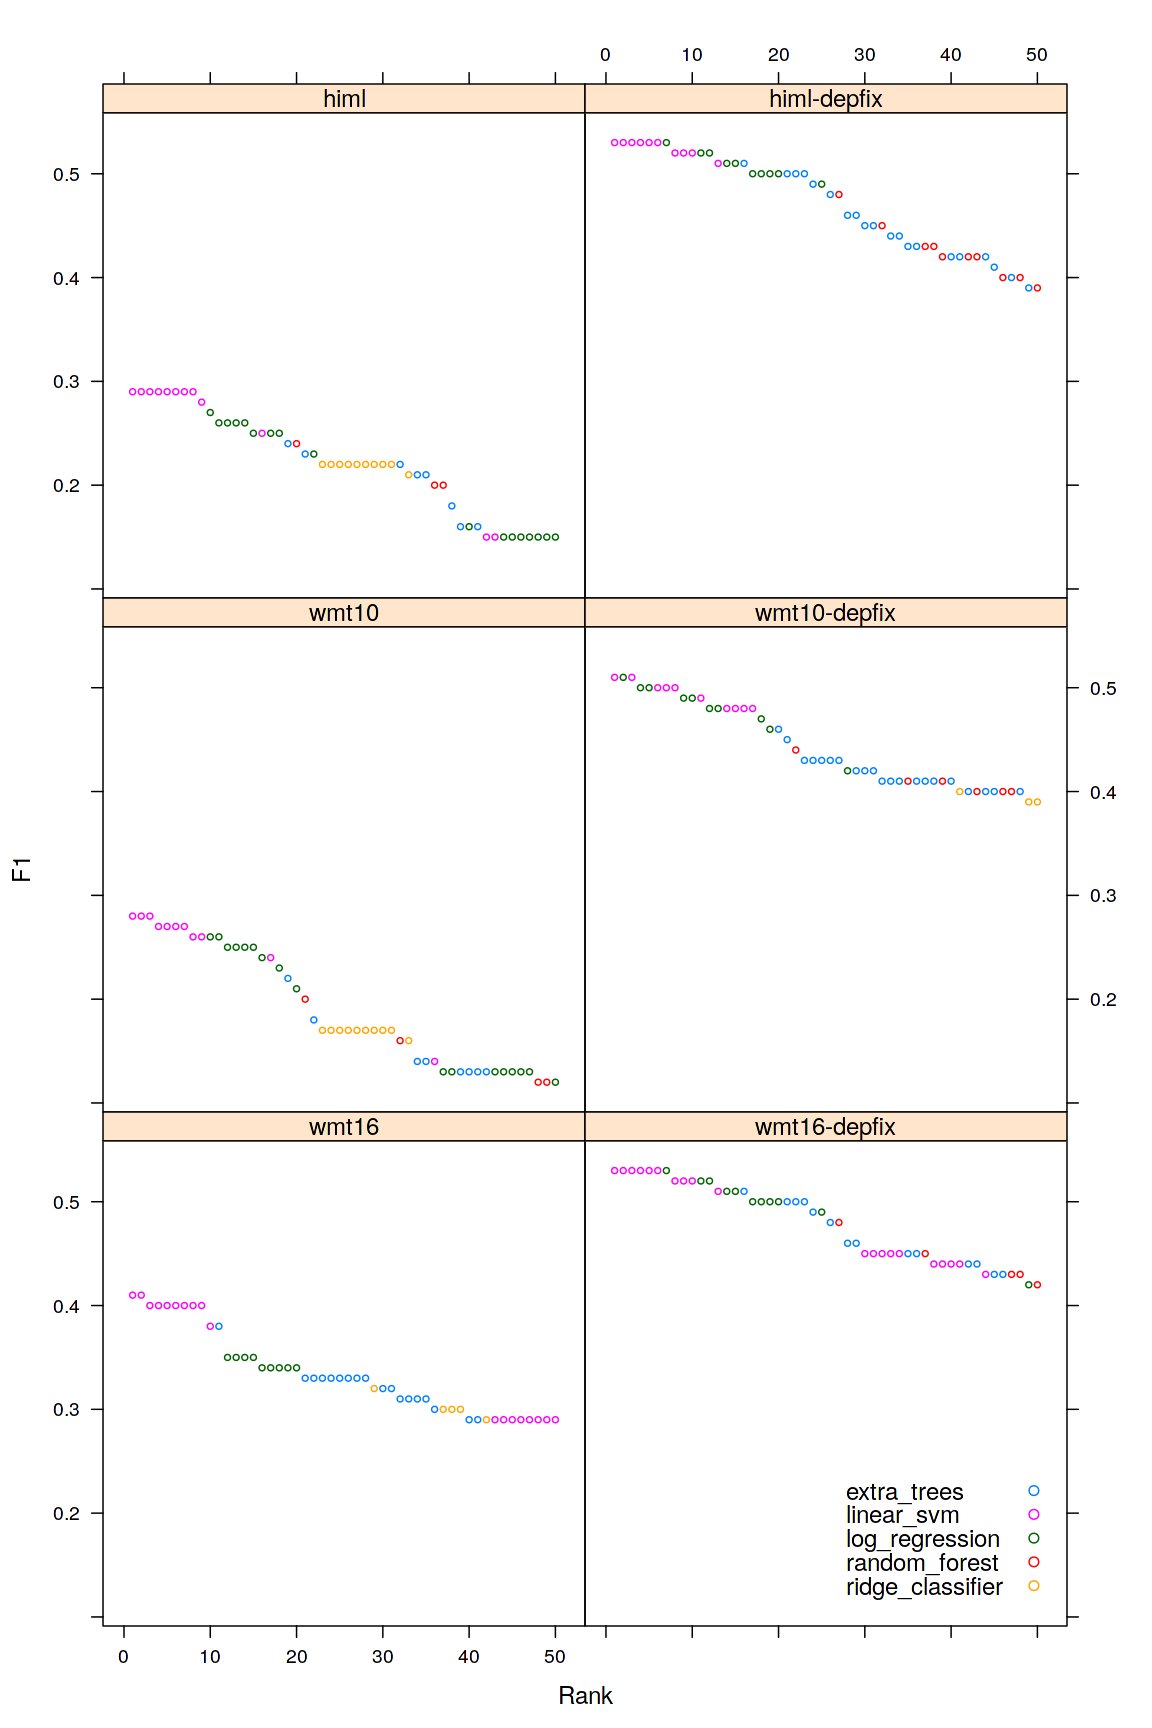
\includegraphics[scale=0.7]{wf-class}
  \caption[ML method comparison - Error detection]{
    Overview of the classifier performance (error detection).
We have tried several variations of the hyperparameters
for each classifier. The classifiers are ordered from the best to the worst. Only top 50 results
are shown for each dataset.
}
  \label{wf-draft}
\end{figure}

\subsection{Feature Selection}

During model comparison, we have compared the performance on two initial feature sets:
one that did not contain any information about the source sentence ($\sim$680 initial features)
and one with source sentence features ($\sim$1360 initial features). Before training,
the features with zero variance were removed, however, no other feature filtering has been
performed. We have noticed that the additional information provided by the source sentence features
significantly improves performance of the majority of the ML methods. Therefore, we have decided
to use this feature set for feature selection method comparison.

Having selected SVM, we tried out several methods for feature
selection and compared their influence on the classifier performance. During the comparison,
we used a SVM model with fixed hyperparameters. We have compared the following methods for
feature selection: KBest selection (with chi-squared scoring function), selection of the percentile
of the features (based on the ANOVA F-test),
selection based on lasso regularization and selection through models with feature importance
scoring (svm, random forest). As far as importance scoring goes, we compared different
model configurations and during features selection, only features with importance higher
than the mean of the feature importance distribution were selected.

The results of feature selection method comparison are shown in~\Fref{wf-sel}. We can see
that most of the time the feature selection performed by either ANOVA percentile selector or
SVM slightly improved the model performance. Therefore, we have decided to use these methods during
the model tuning.

\begin{figure}
\centering
  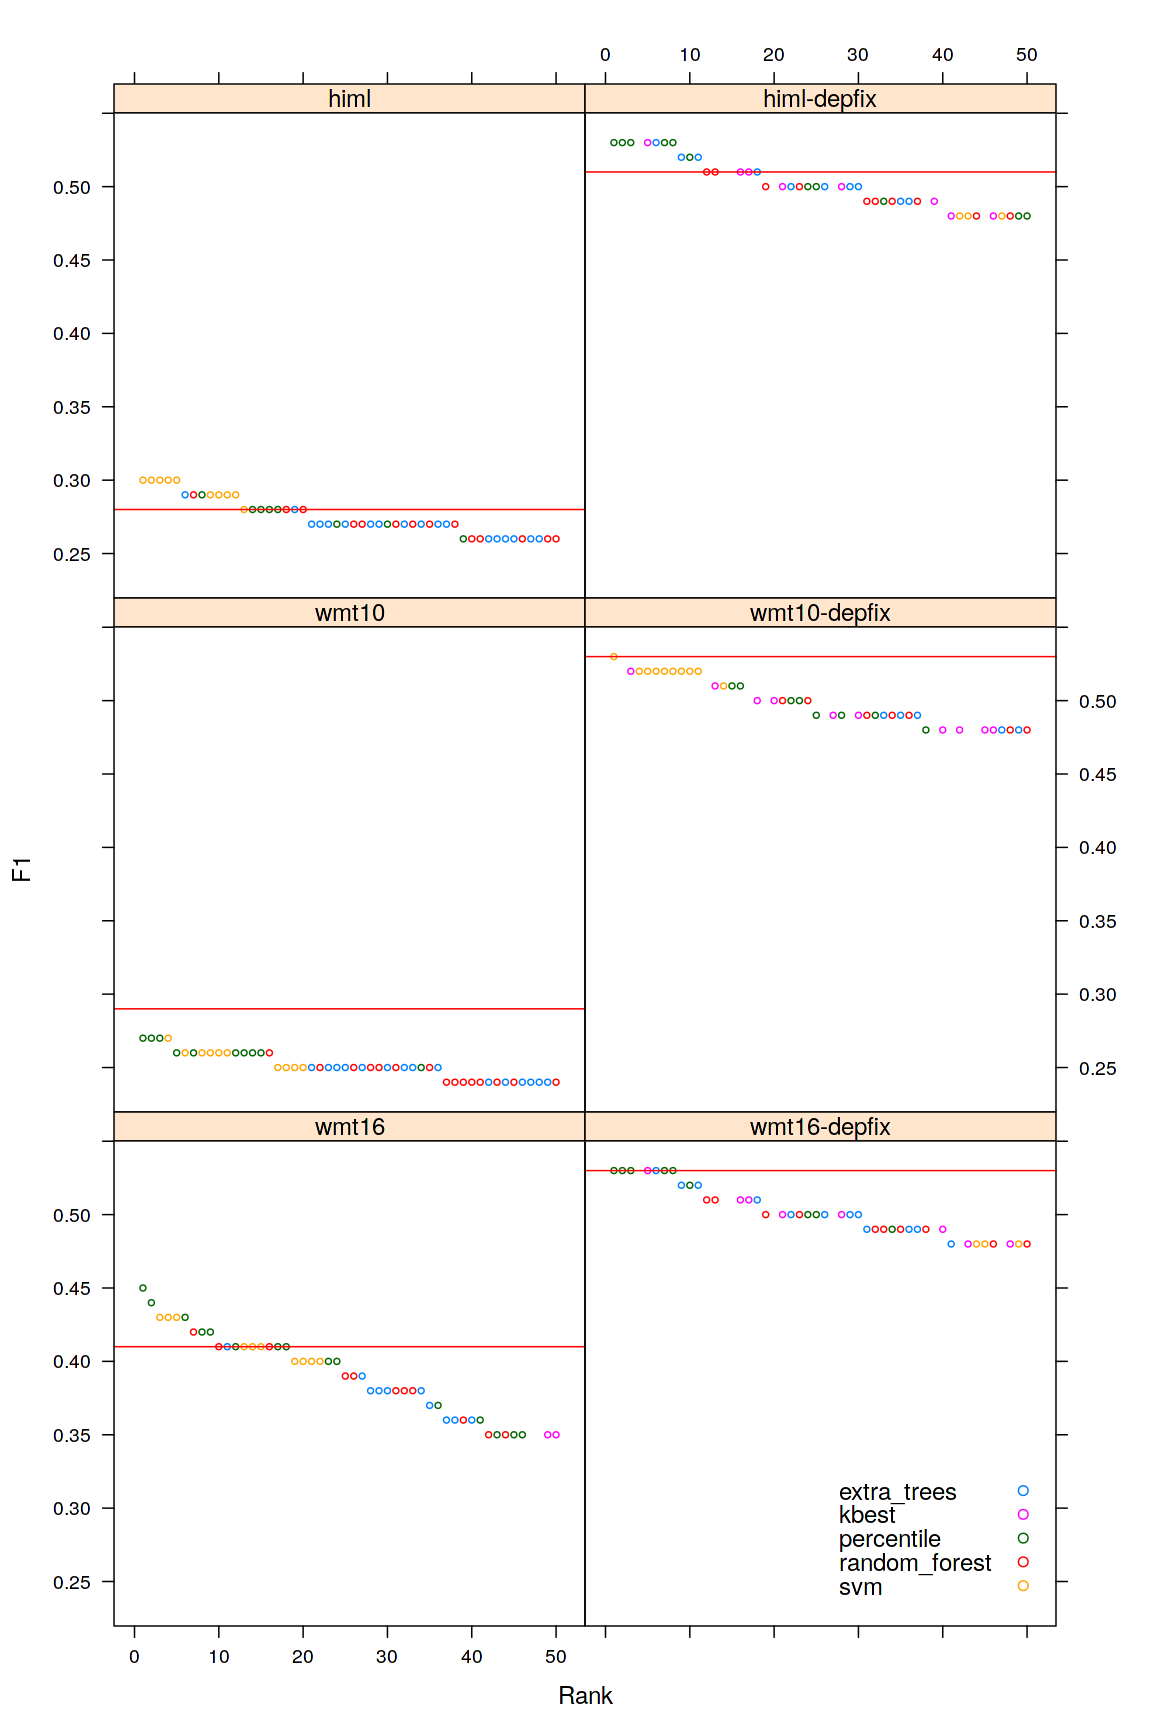
\includegraphics[scale=0.7]{wf-sel}
  \caption[Feature selection method comparison - Error detection]{
    Overview of the performance of the SVM with linear kernel when combined with various feature selection methods.
We have tried several variations of the hyperparameters
for each method. The horizontal line marks the best performance without
any feature selection method. The methods are ordered from the best to the worst. Only top 50 results
are shown for each dataset.
}
  \label{wf-sel}
\end{figure}

%TODO: feature representation - vectorized dicts, binary features???
% chceme to zminovat?

\subsection{Model Summary}

With the ML method and feature selection method chosen, we have proceeded to 
the development of the final model.
We have trained several different models, one for each presented dataset, instead of combining
the datasets and training one larger model. We have chosen this approach because it makes
it easier to exclude specific models if needed (e.g. during final evaluation) and in the
future, include additional models when more training data become available without the need
to retrain the whole error detection component. The use of multiple models for error detection
is described later in Chapter~\ref{chap:eval}.

We present the summary of the trained models in~\Tref{wf-summary}. We can see, that the models
trained on the Depfix data performed better than the ones trained on the original datasets.
Unfortunately, we did not perform any cross-domain evaluation at this stage so we cannot say
that the datasets with Depfix reference sentences provide better training instances for the
error detection models. The better performance might be just a result of more consistent
training data in the corresponding dataset.

The overall
performance is still quite low, so there is still room for improvement. We think that introducing
additional features (e.g. information from the t-layer) or increasing the size of the training data
might help us improve these models in the future.

\begin{table*}[t]
\centering
\small

\begin{tabular}{lll|ccc}
Dataset  &  System  &  Origin  &  Precision  &  Recall  &  F1  \\
\hline
WMT10  &   CU-Bojar  &  REF  &  0.29  &  0.25  &  0.27  \\
HimL  &  Moses  &  PE  &  0.28  &  0.32  &  0.30  \\
WMT16  &  CU-Chimera  &  REF  &  0.40  &  0.44  &  0.42  \\
WMT10  &  CU-Bojar  &  Depfix  &  0.51  &  0.55  &  0.53  \\
HimL  &  Moses  &  Depfix  &  0.55  &  0.51  &  0.53  \\
WMT16  &  CU-Chimera  &  Depfix  &  0.50  &  0.52  &  0.51  \\
\end{tabular}
\caption[Model summary (Czech) - error detection]{
    Summary of the in-domain performance of the trained error detection models. The evaluation was performed
by a jack-knife one-vs-rest classification on each dataset. \pojem{Origin} column indicates origin
of the reference sentences: post-edited (PE), standard reference (REF) or created by Depfix.
}
\label{wf-summary}
\end{table*}


\section{Automatic Morphology Prediction}

The second classification task to predict correct morphological categories for
the words that were marked as incorrect. Because we are using the Interset representation
of morphological features we have several possibilities how to handle this task such
as:
\begin{enumerate}
    \item predict each category separately,
    \item concatenate the features and treat them as a single prediction target,
    \item use the methods that support multitask classification,
\end{enumerate}

With the first option, the biggest issue is determining the order in which the classifiers
should be applied. Additionally, we have to decide if we also want to include the current node's morphological features
into our model's feature set or use the newly predicted ones. The second approach eliminates this problem by predicting the
values simultaneously.
%However, this can quite easily expand the set of the predicted values,
%which usually leads to increase in data sparsity.
This, however considerably enlarges the set of predicted values increasing data sparsity.
This can be a big problem as we have
already shown that the amount of data available for the post-editing task (mainly the post-edited
data) can be quite small. The third option combines the first two by training an estimator
which handles multiple joint classification tasks, one for each morphological category. The
Scikit-Learn toolkit provides several classifiers which support this option.

Before jumping straight into the developing of our classifier, it is important to examine what morphological
changes are made in our training data, how frequently they are made and how can they affect the resulting
surface form generation. For instance, we can predict new values of the \samp{punctype} category,
but it is very unlikely that it will affect the resulting wordform of any of the words
classified as incorrect, because this category is related strictly to punctuation. There are
of course less obvious examples and some categories, while being relevant in one target language
can be pointless in another.

For this reason, we have made a frequency analysis of the changes encountered
in our data, shown in~\Fref{iset-barplot}. We can see that most of the time, only the grammatical
case was modified (more than 50\% of the instances for the Depfix-based datasets and more than 40\% of the instances for
the genuine post-editing datasets). Other changes were a lot less frequent (less than 10\% of the modified instances).
We have also checked, the amount of modifications made for individual general POS classes.
\Tref{changes-pos} summarizes the modification frequencies for each
POS class. In conclusion, we have decided to focus on predicting the following categories: grammatical case, number, gender
and animateness. These categories are relevant to the majority of the changed words, therefore, changes made by
a classifier predicting these categories should be noticeable.

\begin{table*}[t]
\centering
\small

\begin{tabular}{lc}
POS  &  Frequency  \\
\hline
noun    &   38\%  \\
adj     &   16\%  \\
adp     &   10\%  \\
verb    &   9\%  \\
adv     &   9\%  \\
\end{tabular}
\caption{
    Change frequency of various POS classes in Czech.
}
\label{changes-pos}
\end{table*}


\subsection{Machine Learning Method Comparison}

We have decided to train four different types of model: one predicting case only (C), one predicting case and number (CN),
 one predicting case, number and gender (CNG) and one predicting case, number, gender and animateness (CNGA).
We have used the same datasets as in the previous task, however, this
time we have extracted only feature vectors of the instances that were marked as incorrect in our training data. Since
our predictors classify only the incorrect instances, training them on the whole dataset would only create
unnecessary bias. On the other hand, this has made the training sets quite small (containing only a few hundreds of examples
at most). The summary of the training data is in~\Tref{cats-training-sum}. We have decided to train a separate classifier
for each dataset instead of combining the data together, because we can simply combine the models instead (e.g. via majority
vote, best prediction etc.). This allows us to evaluate the combined model on a test set of our choice.
%simply by leaving
%out the model which was trained on that specific test set.
We can also leave out the model trained (using jack-knife) on that particular test set, to see the applicability across test sets or domains.

\begin{table*}[t]
\centering
\small

\begin{tabular}{lll|c}
Dataset  &  System  &  Origin  &  \hash{} training instances  \\
\hline
WMT10  &  CU-Bojar  &  REF  &  645  \\
HimL  &   Moses  &  PE  & 338  \\
WMT16  &  CU-Chimera  &  REF  &  722  \\
WMT10  &  CU-Bojar  &  Depfix  &  210  \\
HimL  &  Moses  &  Depfix  &  72  \\
WMT16  &  CU-Chimera  &  Depfix  &  99  \\
\end{tabular}
\caption[Summary of the extracted Czech training data for morphological prediction]{
    Summary of the size of the training data extracted from various datasets translated by different SMT systems.
	\pojem{Origin} column indicates origin
	of the reference sentences: post-edited (PE), standard reference (REF) or created by Depfix from the given MT output.
}
\label{cats-training-sum}
\end{table*}

Again, we had to decide which ML method should we use for this task. 
We have examined similar set of classifiers with similar
hyperparameters as in the error classification task to get a rough idea about their capabilities.
We have considered using the F-measure again, however, due to the nature of the training data (all
instances are classified), the model accuracy metric seemed more informative.
A rough comparison was made with the case classifier only.
Adding additional targets to the classifiers naturally lowers their overall accuracy,
however, their performance have been similar with respect to each other
The results are shown in~\Fref{cats-draft}. We can see, that even without any sophisticated parameter
tuning or feature filtering, the classifiers perform quite well. We can also notice that in most of the cases, the ensemble
methods (mainly extremely randomized trees) performed slightly better than the rest of the examined ML methods. Therefore, we have decided
to pick this method for further experiments.

\begin{figure}
\centering
  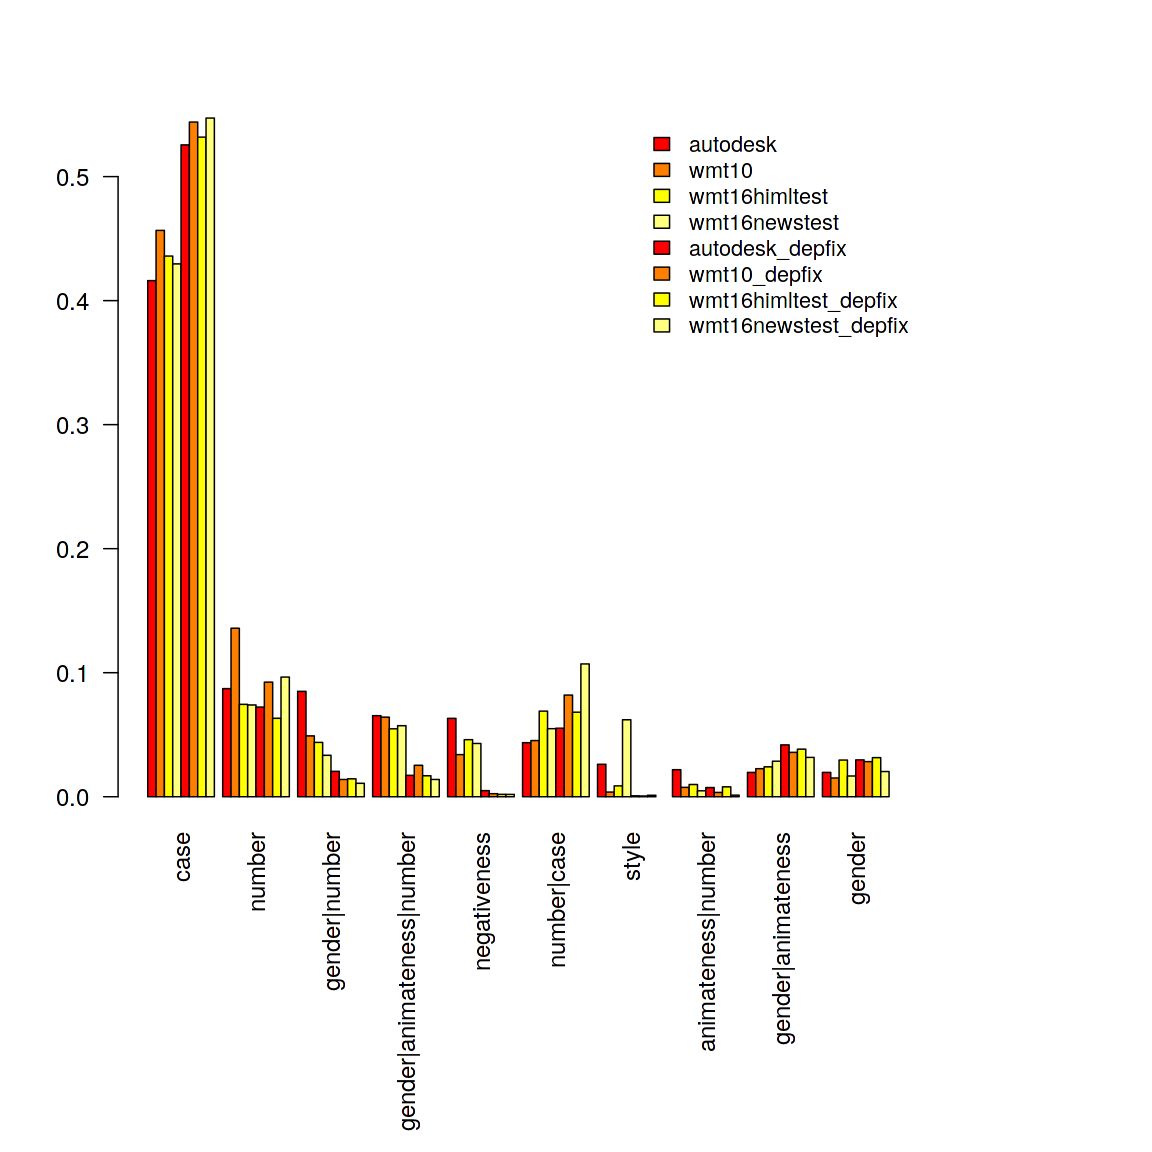
\includegraphics[scale=0.7]{iset}
  \caption[Change frequency of Czech morphological categories]{
    Frequency of the most changed Interset categories, grouped by a datasets. Categories containing
    "\textbar" symbol (e.g. gender\textbar{}number) represent changes made simultaneously.
}
  \label{iset-barplot}
\end{figure}

% with source
\begin{figure}
\centering
  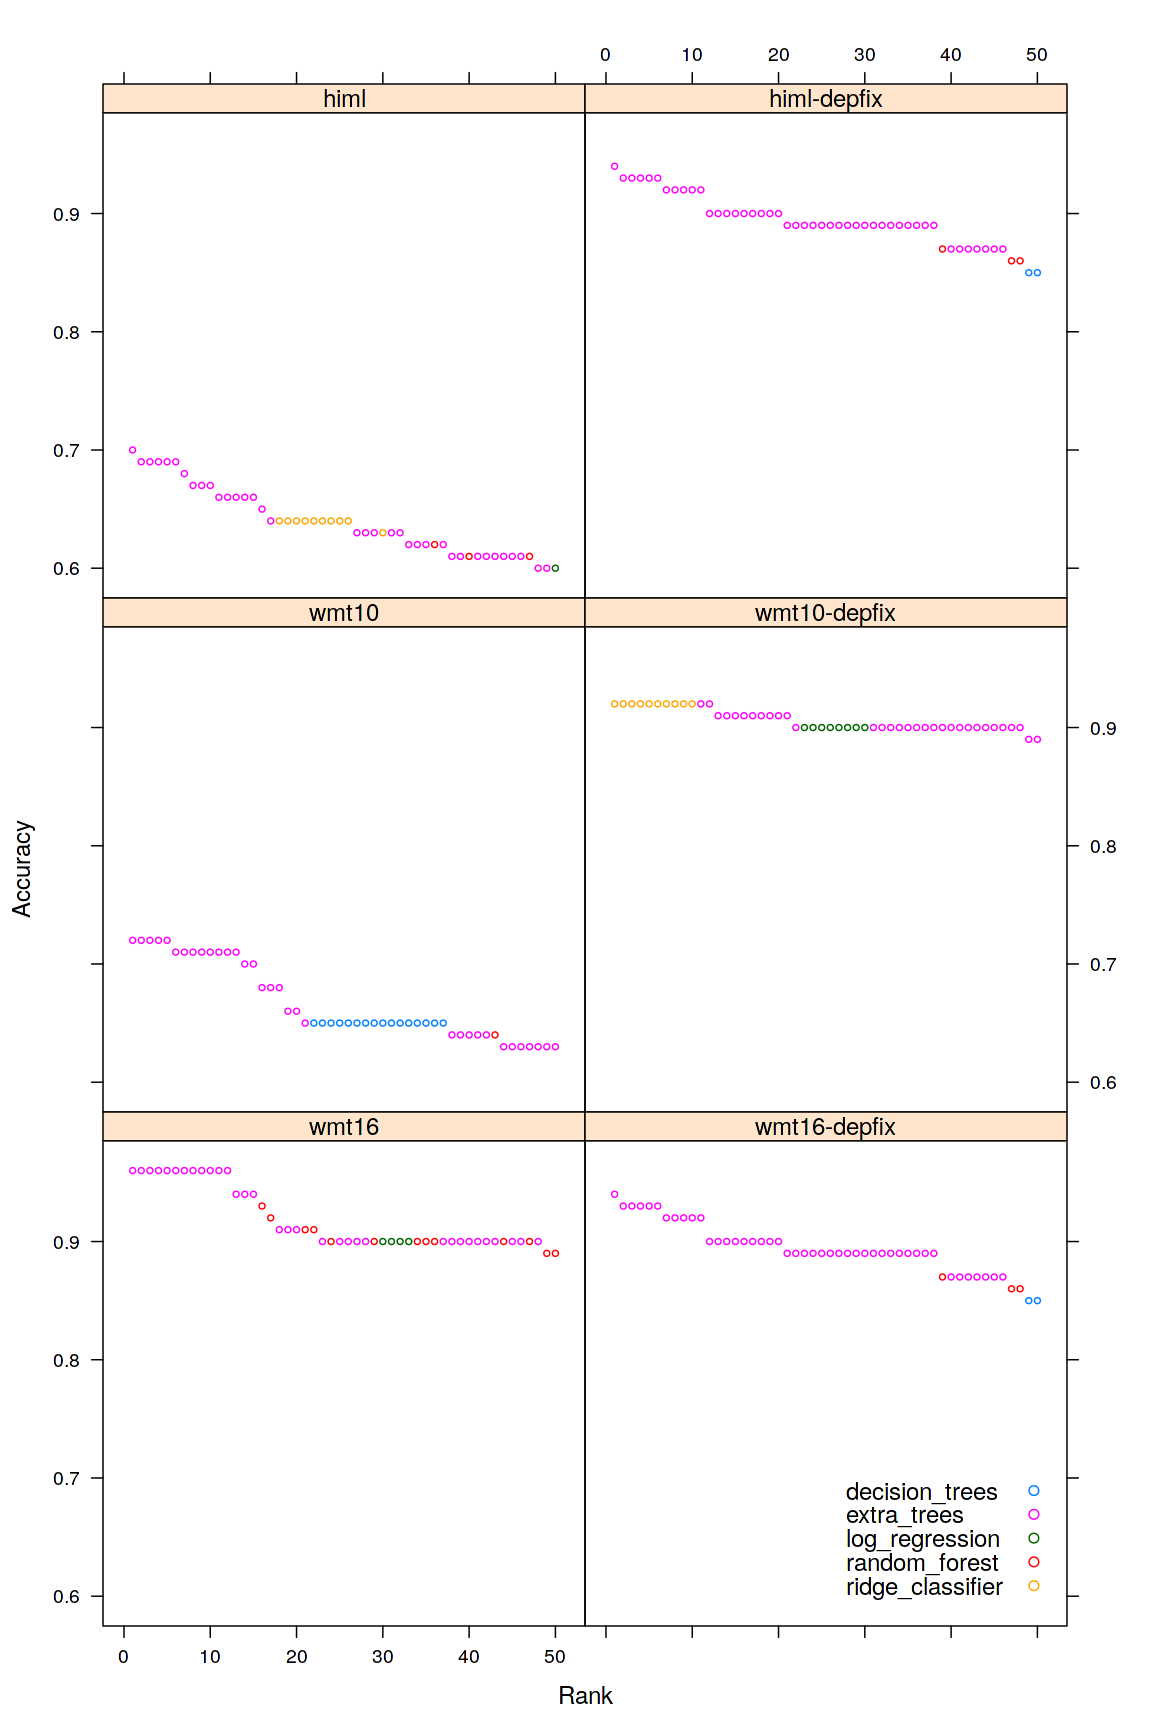
\includegraphics[scale=0.7]{cats-class}
  \caption[ML method comparison - Morphological prediction]{
    Overview of the classifier performance (category prediction).
We have tried several variations of the hyperparameters
for each classifier. The classifiers are ordered from the best to the worst. Only top 50 results
are shown for each dataset.
}
  \label{cats-draft}
\end{figure}

\subsection{Feature Selection}

We have decided to perform additional feature selection with models trained on the standard HimL dataset
and WMT10 dataset because there is still a reasonable room for an improvement. Again, we have tried two initial feature
sets, one using the source side features and one without them. We have not noticed any significant difference in performance
between the models trained on these two initial feature sets so we decided to use the larger one and leave
the feature selection to the automatic feature selection method. Additionally, probably due to the nature of the classifier, we have noticed
another slight improvement by adding the \pojem{source lemma} (both of the aligned node and its parent) features, so we have also
included them to the initial feature set.\footnote{We have not included the \pojem{MT lemma} feature, because we wanted to
try using models trained on Czech for German post-editing and this feature is too language-specific for that purpose.}

We have compared several methods of feature selection: KBest selection
(with chi-squared scoring function), selection based on lasso regularization and selection through
models (svm, random forest). Again, we have done a rough comparison of these methods by trying out
several hyperparameter configurations. We tested them on a model with fixed parameters. The result summary
is in~\Fref{cats-sel}. We can see that regarding HimL dataset, feature selection did not have
any positive effect on the resulting performance. On the other hand, we have decided to use the SVM-based
feature selection for the WMT10 dataset model training.

\begin{figure}
\centering
  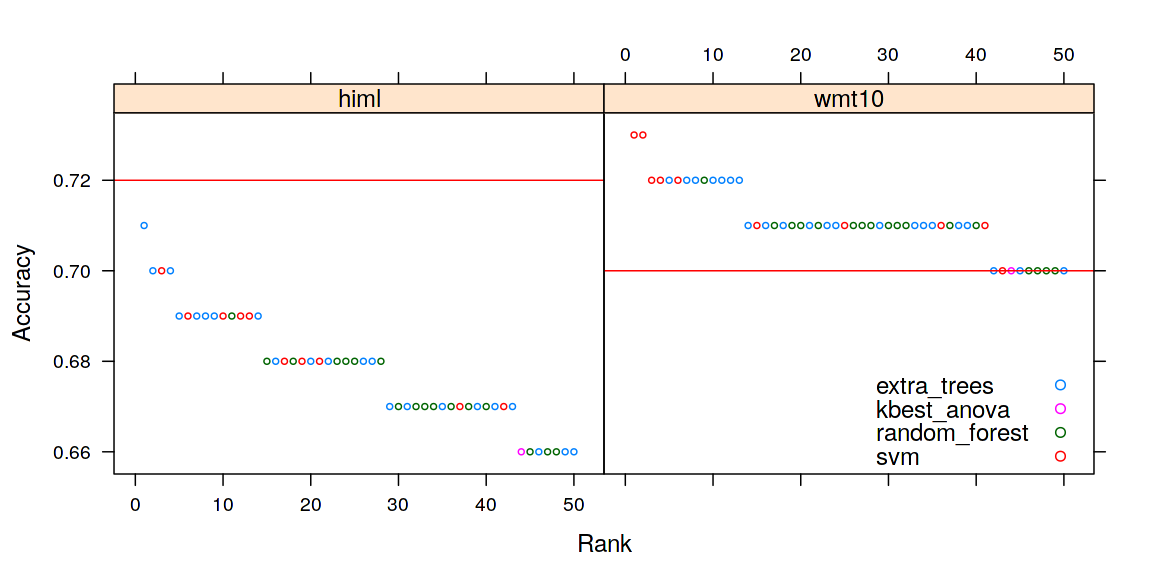
\includegraphics[scale=0.7]{cat-sel}
  \caption[Feature selection method comparison - Morphological prediction]{
    Overview of random forest performance when combined with various feature selection methods.
The methods are ordered from the best to the worst. The horizontal line indicates the best performance without
any feature selection method. Only top 50 results are shown for both examined datasets.
}
  \label{cats-sel}
\end{figure}

%\subsection{Multitask models}
%todo???

\subsection{Model Summary}

In the end, we have trained six different models, one for the each dataset presented in the rough comparison.
Aside from the case classifier, we have also compared performance of the chosen multitask classifiers:
the case-number (CN), the case-number-gender (CNG) and the case-number-gender-animateness (CNGA)
classifier. These classifiers were trained using the same ML methods, each one was tuned separately.
The summary of the final in-domain performance is in~\Tref{cats-summary}.

We can see that by including additional target for the multitask classification the accuracy of the trained
model becomes naturally lower. However, we must take into account that we have only classified the predicted
values as correct or incorrect and we have not distinguished partially correct predictions. Brief overview
of the categories predicted by the CNGA classifier has shown us that usually a predictor misclassifies only
one or two of the target categories. Another thing to keep in mind is the fact, that even though the predicted
categories might not be equal to the gold standard, the generated surface form might still match the reference form
due to the morphological ambiguities of the language. For these reasons, we decided to use all these models during the system evaluation.

%Surprisingly, accuracy of the multitask models trained on WMT16 dataset dropped significantly when training a
%more complex classifier, underperforming even the baseline predictor. It is possible that the chosen ML
%method is not suitable for this dataset, even though it is performing well with the simple case classifier.

\begin{table*}[t]
\centering
\small

\resizebox{0.98\textwidth}{!}{
\begin{tabular}{lll|cccc}
Dataset  &  System  &  Origin  &  Case (Base)  &  CN (Base)  & CNG (Base)  &  CNGA (Base)  \\
\hline
WMT10  &  CU-Bojar  &  REF  &  73\% (35\%)  &  53\% (14\%)  &  40\% (7\%)  &  37\% (7\%)  \\
HimL  &  Moses  &  PE  &  72\% (34\%)  &  50\% (11\%)  & 41\% (5\%)  &  41\% (4\%)  \\
WMT16  &  CU-Chimera  &  REF  &  95\% (50\%)  &  45\% (21\%)  &  34\% (10\%)  &  32\% (10\%)  \\
WMT10  &  CU-Bojar  &  Depfix  &  92\% (45\%)  &  83\% (22\%)  &  69\% (19\%)  &  69\% (19\%)  \\
HimL  &  Moses  &  Depfix  &  92\% (47\%)  &  78\% (26\%)  &  73\% (23\%)  &  71\% (23\%)  \\
WMT16  &  CU-Chimera  &  Depfix  &  93\% (54\%)  &  64\% (16\%)  &  56\% (11\%)  &  53\% (9\%)  \\
\end{tabular}
}
\caption[Model summary (Czech) - morphological prediction]{
    Summary of the in-domain accuracy of the trained morphological prediction models. The evaluation was performed
by jack-knife one-vs-rest classification of the each dataset. Performance of the baseline (Base)
classifier is presented for comparison.
\pojem{Origin} column indicates origin
of the reference sentences: post-edited (PE), standard reference (REF) or created by Depfix.
}
\label{cats-summary}
\end{table*}

%\todo{tohle az do final evaluace?}
%Since the domains of the datasets differ to a various degrees, we have decided to combine the models trained
%on the different datasets, however, we do not combine different types of classifier. This combined model
%compares result of each separate classifier (with the prediction probability) and picks the most probable choice.

